% this file is called up by thesis.tex
% content in this file will be fed into the main document

%: ----------------------- name of chapter  -------------------------
\chapter{Background}\label{background} % top level followed by section, subsection


%: ----------------------- paths to graphics ------------------------

% change according to folder and file names
%\graphicspath{{2-Consorzi/images/}}


%: ----------------------- contents from here ------------------------
To fully understand how M2MShare works and what kind of simulator have to be used to emulate it, is worth to take a look at some technology backgrounds which can be useful to know before go further to the following of the thesis. In this chapter we describe what a DTN is, the notion of peer-to-peer and overlay networks.

\section{Delay/Disruption Tolerant Networks (DTN)}
The Internet is a connected network where internet protocols, most notably transmission control protocol/internet protocol (TCP/IP), are dependent upon (low) latencies of approximately milliseconds. This low latency, coupled with low bit error rates, allows TCP to reliably transmit and receive acknowledgements for messages traversing the terrestrial Internet. 
\\

A DTN is a network designed to operate effectively in highly-challenged environments where protocols adopted in connected networks (i.e. TCP/IP) fail. The "D" part in DTN acronym stands both for \textit{Delay} and for \textit{Disruption}. By delay we mean the end-to-end latency of data transmission. Some of those delays are inherent in the transmission medium, or the geometry of the system, but others are due to packets being temporarily stored on intermediate nodes. By disruption, we mean factors that cause connections to break down, or not be established, normally due to transient or quickly changing aspects of the system and/or its environment.
\\

There are some environments where low latency and end-to-end links are rarely available. One of the best examples of high latency with intermittent connectivity is that of space communications \cite{Burleigh2003365}. One-way trip times, at the speed of light, from the Earth to the Moon incurs a delay of 1.7 seconds; while one-way trip times to Mars incur a minimum delay of 8 minutes. The problem of latency for interplanetary links is exasperated with increased error rate due to solar radiation. In addition, the celestial bodies are in constant motion, which can block the required line-of-sight between transmit and receive antennas, resulting in links that at best are only intermittently connected. 
\\

DTNs need not be solely concerned with deep-space communications but can also be useful in terrestrial networks. In some environment, networks may be subjected to high disruption probability. One example is military application, where adopting DTNs allows the retrieval of critical information in mobile battlefield scenarios using only intermittently connected network communications. Another application, more peaceful, is the adoption of DTNs to overcome a major natural disaster. In such a situation terrestrial infrastructures may have been swept away and tolerant protocols must be used to coordinate rescue teams.  
\\
Networks adopted in these situations are characterized by:
\begin{itemize}
\item \textbf{Intermittent Connectivity:} if there is no end-to-end path between source and destination, end-to-end communication using the TCP/IP protocols does not work.
\item \textbf{Long or Variable Delay:} in addition to intermittent connectivity, long propagation delays between nodes and variable queuing delays at nodes contribute to end-to-end path delays that can defeat Internet protocols and applications that rely on quick return of acknowledgements or data.
\item \textbf{Asymmetric Data Rates:} the Internet supports moderate asymmetries of bidirectional data rate for users with cable TV or asymmetric DSL access. But if asymmetries are large, they defeat conversational protocols.
\item \textbf{High Error Rates:} bit errors on links require correction (which requires more bits and more processing) or retransmission of the entire packet (which results in more network traffic). For a given link-error rate, fewer retransmissions are needed for hop-by-hop than for end-to-end retransmission.
\end{itemize}

To overcome problems associated with all these factors, DTNs use a old yet affective method used in postal systems since ancient times. In this method, named \textit{Store-and-forwarding}, node physically delivers data to the destination moving from the source location to the destination of the recipient node (\figurename~\ref{fig:store-carry-forward}). Replication techniques can be adopted to increase the deliver ratio, copying the carried data and giving it to other nodes following a different physical path.

\begin{figure}[htpb]
  \begin{center}
    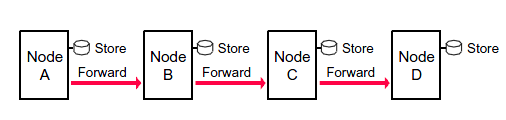
\includegraphics[scale=0.6]{2-background/img/store-and-forward.png}
    \caption{\textit{Store-and-forwarding} technique example}    
    \label{fig:store-carry-forward}
  \end{center}
\end{figure}

Messages are stored in storage mediums which can hold them for a long time period called persistent storage. This is another difference with internet protocols, where routers adopt very short-term storage provided by memory chips to store incoming packets. In Internet routers messages are queued only for a few milliseconds while they are waiting for their next hop. In DTNs routers need persistent storage for one or more of the following reasons:
\begin{itemize}
\item A communication link to the next hop may not be available for a long time and during this period message must be stored in the router.
\item There could be asymmetries in speed and reliability between nodes, so one node in a communicating pair may send or receive data much faster or more reliably than the other node.
\item A message, once transmitted, may need to be retransmitted if an error occurs at an upstream node or link, or if an upstream node declines acceptance of a forwarded message.
\end{itemize}

For more insight about DTNs researches, refer to \cite{dtnResearch}.

 
\section{Peer-to-Peer networks}
The most distinctive difference between Client/Server networking and Peer-to-Peer (P2P) networking is the role of each node in the network. In Peer-to-Peer networks nodes act as Servent, which is is an artificial word derived from the terms server and client. This term represent the capability of the nodes of a Peer-to-Peer network of acting at the same time as server as well as a client. In Client/Server networks each node can act as a server or as a client but cannot embrace both capabilities.
\\

In \cite{Aberer02anoverview} are identified three principles underlying P2P networks:
\begin{itemize}
\item  \textbf{Principle of sharing resources}: P2P systems involve an aspect of resource sharing, such as disk space network bandwidth or services. By sharing of resources applications can be realized which could not be set up by a single node.
\item \textbf{Principle of decentralization}: this is an immediate consequence of sharing of resources. Parts of the system or even the whole system are no longer operated centrally. Decentralization is in particular interesting in order to avoid single-point-of-failures or performance bottlenecks in the system.
\item \textbf{Principle of self-organization}: when a P2P system becomes fully decentralized then there exists no longer a node that can centrally coordinate its activities or a database to store global information about the system centrally. Therefore nodes have to self-organize themselves, based on whatever local information is available and interacting with neighbours nodes.
\end{itemize}




\subsection{Peer-to-Peer networks as Overlay networks}
Peer-to-peer networks are typically constructed as overlay networks. These are computer networks which are built on top of other networks, adding an additional level of routing-logic. This is often done in the application layer, above transport and network layers, where maintenance and management algorithms operate. Overlays usually define some set of functions to forward overlay packets. In order to implement such a higher-level of routing, many overlay networks define an additional level of logical routes above routes provided by the network layer. Each logical route can be composed by multiple lower-levels routes, i.e. routes composed by several IP-level routes.
\\

Overlay networks provide design flexibility and ease of deployment, at the cost of little inefficiency compared to a system implemented directly in coordination with the network layer. Also, designing a system using overlays helps to focus on the problem and functionalities to provide. While overlays are positioned at the application layer, it is possible to think to them as a distinct layer implementing higher-lever routing and transport services, while the complexities of network-level routing and transport are encapsulated in the lower layers.
\\

This allows to implement new services that are not yet available within the existing network. Some examples are the Distributed Hash Table (DHT) or the implementation of Virtual Private Networks (VPNs). 


%It also separates design concerns. Indeed, while overlays are positioned at the application layer, it is more fitting to think of them as a distinct layer implementing higher-lever routing and transport services. This separation of concerns partially decouples design, implementation, and optimization from the network and transport layer. The programmer is then free to focus solely on whatever problems are at hand, while the complexities of network-level routing and transport are encapsulated in the lower layers.
%\\

%The use of an overlay network in the design of new Internet services bypasses the need for strong social coordination during deployment. This has proven important in the continued evolution of the network, as individual autonomous systems and end-users can begin (or end) providing services in a piece-wise fashion. Multicast serves as a strong example of why such piece-wise role out is critical for eventual deployment.

\subsection{Peer-to-Peer architectures}
One ways to classify P2P networks is to consider the degree of centralization of the network and divides P2P networks in centralized or decentralized (or unstructured) networks.
\\

\paragraph{Centralized P2P networks} 
In \cite{Schollmeier:2001:DPN:882470.883282}, R. Schollmeier defines Peer-to-peer networks and algorithms in which an essential subset of peers exists as \textit{hybrid} P2P networks. Hybrid networks typically have one or more strongly differentiated roles for various subsets of peers. Often role differentiation is related to the class of resource being shared. For example, one set of peers may handle storage, and another provide computational power. One of the most famous occurrence of the P2P paradigm was probably Napster\cite{Carlsson:2001:RFN:647728.734520}. This file-sharing system used an architecture in which a centralized entity provides a directory service to all participating peers, effectively forming a star network. All peers joining the system have to register their data with this centralized server. This allows other peers in the system to locate any data in the network by presence of a physically centralized directory. Only pointers to decentralized available peers are stored at the centralized server while the actual data is store in peers. When a peer found a pointer to relevant data in the directory, it could directly communicate with other peers that store the data in a decentralized manner, completely bypassing the centralized directory entity. Napster cannot be denoted as a pure P2P system because without central directory servers, single peers are not able to find resources shared by other peers.
\\

\paragraph{Decentralized P2P networks}
In decentralized (or unstructured) P2P architectures peers do not rely on any centralized entity to locate data items within the network. R. Schollmeier defines such type of networks as \textit{pure} P2P networks \cite{Schollmeier:2001:DPN:882470.883282}. In these networks any peer in the underlying topology can be added and removed arbitrarily without having the network suffering any loss of network service. More specifically, in decentralized P2P networks, peers recursively forward received requests to neighbouring peers, in an attempt to find all relevant items in the network. This request forwarding is done using a broadcast technique know as message flooding. To prevent infinite loops and to control the number of messages generated by one single request, each message gets assigned a time-to-live (TTL) value. Each peer forwarding such a message decreases this value by one, and only messages with positive TTL values get forwarded. The main advantage of unstructured P2P networks is the fact that there is no need to maintain a network structure, as peers maintain only pointers to a limited number of direct neighbours. Also there is no need for a specific storage location for data items, as they can be located anywhere in the network.
\\

%In \cite{Schollmeier:2001:DPN:882470.883282}, R. Schollmeier splits P2P networking
%definition into two sub-definitions: \textit{pure} and \textit{hybrid} Peer-to-Peer networks.\\ 
%The network is said pure if any peer in the underlying topology can be added and removed arbitrarily without having the network suffering any loss of network service. In other words, there is no special set of nodes that must be present for the service to work. \\
%Peer-to-peer networks and algorithms in which an essential subset of peers exists are said to be hybrid networks. Hybrid networks typically have one or more strongly differentiated roles for various subsets of peers. Often role differentiation is related to the class of resource being shared. For example, one set of peers may handle storage, and another provide computational power. \\
%%In other networks roles are differentiated across functionality, as is done in peer-to-peer file-sharing services such as Napster and BitTorrent, both of which separate indexing, and storage and download.
%Pure peer-to-peer networks tend to generalize better, since they do not require any centralized, essential node to provide the related service.

\section{Case study: BlueTorrent}
BlueTorrent \cite{bluetorrent} is a pure peer-to-peer protocol which enables file transfer among mobile nodes using Bluetooth. The Bluetooth channel tends to be error-prone in the urban streets due to multipath, WiFi interference etc. In addition, the short communication range and mobility of users result in short link/contact duration. BlueTorrent shares contents by using file swarming, mainly due to the limited bandwidth and the short contact duration. We now describe the core components of BlueTorrent, shown in \figurename~\ref{fig:bluetorrent}.

\begin{figure}[htpb]
  \begin{center}
    \includegraphics[scale=0.6]{2-background/img/bluetorrent.png}
    \caption{BlueTorrent architecture \cite{bluetorrent}}    
    \label{fig:bluetorrent}
  \end{center}
\end{figure}

\paragraph{Peer Manager}
This module manages physical neighbours among which it tries to choose the best peer. In BlueTorrent, a node keeps track of connections for efficient peer selection, by logging connection frequency and duration. The main purpose is to rank the physical neighbours by using the connection frequency/duration, giving more chances to those freshly encountered nodes. BlueTorrent uses nodes distance to evaluate the contact duration with a neighbour node. The idea is that is preferable to select a peer that has the longest residual contact duration, which can be calculated by the direction/distance among peers. The module uses RSSI values of the inquiry responses to estimate the distance among peers and considers these distance values as the first criterion for peer selection. A way to estimate distances using RSSI values is shown in \cite{positionBluetooth}.

\paragraph{Query Processor}
Before a peer can download some content from another peer, it is fundamental that it knows where this content is. Content can be searchable through indices which include a unique ID, title, producer, media type, etc. BlueTorrent is equipped with a lightweight database for such index management and search. When a user is looking for a particular content, it can express his request as a simple query string. Whenever a node discovers another node, it first sends the query. Upon receiving a query, the target node will look up its database to find an exact match of keys, this match will be automatically reported to the query originator, and the user may decide whether to initiate downloading using the ID of the content.

\paragraph{Data Collector}
BlueTorrent shares contents by using file swarming. Each data source divides a file into \textit{K} pieces or blocks, each of them can be individually downloaded. Each node has a bitmap of the available pieces for efficient piece reconciliation. Whenever a connection is available, peers first exchange their bitmaps to find out missing pieces through simple bit operations. The size of a typical bitmap is very small and the related overhead is negligible. When only one party has data to transfer, it uses asymmetric mode whereas a symmetric mode is used when both have data to transfer. The size of a piece is selected based on the characteristics of Bluetooth bandwidth and mobility patterns. 




% ---------------------------------------------------------------------------
%: ----------------------- end of thesis sub-document ------------------------
% ---------------------------------------------------------------------------

